\chapter{Metodología}

\section{Análisis general de la plataforma}
Se realizó un análisis general de la herramienta para conocer enteramente con qué nos encontramos, en qué plataforma está basada y si se han realizado desarrollos adicionales sobre la misma para adecuarlo a las necesidades de la UGR.

\section{Entrevistas personales}

Para recoger la mayor información posible sobre las opiniones de los usuarios de Prado2 se realizaron una serie de entrevistas personales de carácter informal con profesores, alumnos y administradores y así poder hacer una valoración global del estado actual de la plataforma, teniendo en cuenta a todos los actores implicados en la misma.

\bigskip
Algunas de estas entrevistas incluyeron un test de usabilidad que consistía en pedir a los usuarios que realizaran una tarea sencilla y ver cuánto tiempo tardaban en realizarla. 

\bigskip
Dicha tarea consistía en pedirles cambiar la imagen del perfil de Prado2. El test se basó en el test de usabilidad planteado por Steve Krug en su libro \textit{Don't make me think} \cite{stevekrug} y se pedía que partiendo de una página neutra, como puede ser la pagina de inicio de un buscador, entraran en Prado2 y localizaran desde donde podían cambiar su imagen de perfil.


\section{Encuesta a los usuarios}
Uno de los actores más importantes de cualquier plataforma web son sus usuarios por lo que queríamos conocer de primera mano sus opiniones, para ello se preparó un breve cuestionario online que fue difundido a través de la lista de correo general de la UGR.

\bigskip
La encuesta se realizó con la herramienta \texttt{Google Forms} y estuvo activa desde el 14 de Marzo hasta el 10 de Mayo de 2017, los primeros días se le dio difusión a través de grupos de mensajería y redes sociales. El 21 de Marzo se envió a la lista de correo infoUGR de la Universidad por parte del Tutor y el 23 de Marzo la DEIIT nos hizo el favor de enviarla a la comunidad de estudiantes de la ETSIIT ya que la lista infoUGR al estar en un buzón propio no suele tener la difusión que tienen los mensajes que van a la bandeja de entrada.

\bigskip
Dicho cuestionario constaba de varias preguntas preguntas cerradas de respuesta múltiple, ya que las mismas son más objetivas a la hora de hacer un análisis estadístico, también se incluyeron tres preguntas opcionales de respuesta abierta para que los usuarios pudieran exponer razonadamente sus opiniones.

Las preguntas eran las siguientes:

\begin{enumerate}

  \item \textbf{Selección del tipo de usuario} Se pregunta si el usuario es Estudiante, Profesor u otro tipo de miembro de la comunidad universitario, como por ejemplo, doctorandos.

  		\shadowbox{
\includegraphics[width=0.9\textwidth]{../screenshots/poll/01}}

  \item \textbf{Selección de la titulación} Se pregunta la titulación del usuario, ya que vimos que las opiniones variaban en base a la misma, el listado oficial de titulaciones lo obtuvimos del Portal de Transparencia de la UGR \url{http://transparente.ugr.es/}

  \shadowbox{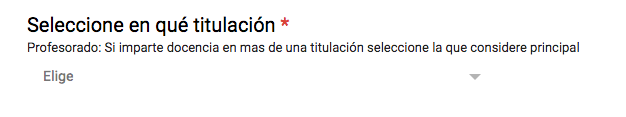
\includegraphics[width=0.9\textwidth]{../screenshots/poll/02}}

  \item \textbf{¿Con qué periodicidad accede a Prado2?} Es interesante saber  la periodicidad con la que los usuarios acceden a la plataforma, para además cotejarla con el análisis de los registros de moodle

  \shadowbox{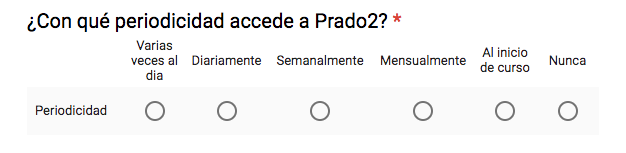
\includegraphics[width=0.9\textwidth]{../screenshots/poll/03}}

  \item \textbf{Califique las siguientes opciones según sus necesidades} Presentamos al usuario una serie de opciones de la plataforma extraídas de valoraciones personales de varios usuarios, dichas opciones son:

  		\begin{itemize}
  			\item \textbf{Acceso desde dispositivos móviles} La mayor parte de las quejas recibidas antes de empezar este proyecto era la dificultad para acceder desde dispositivos móviles y la falta de una aplicación nativa para dichos dispositivos.
  			\item \textbf{Insignias} Implementación del sistema de insignias de Mozilla Open Badges para otorgar a los alumnos reconocimiento digital de sus cualidades y logros.
  			\item \textbf{Blog de la asignatura} Permitir a las asignaturas mantener un blog dentro de la plataforma, dicho blog solo está accesible para los alumnos de la asignatura.
  			\item \textbf{Blog de los alumnos} Permitir a los alumnos mantener un blog dentro de la plataforma, las publicaciones de dicho blog se pueden configurar para que sean visibles solo para otros alumnos de la misma asignatura o para todos los usuarios de la plataforma.
  			\item \textbf{Mensajería interna} Se debe permite la comunicación entre profesores y alumnos sin salir de la misma.
  			\item \textbf{Estadísticas de uso} Permitir a los alumnos y profesores acceder a las estadísticas de uso de la plataforma.
  			\item \textbf{Calificaciones} Permitir a los alumnos acceder a las calificaciones de sus tareas y exámenes de la asignatura.

		\end{itemize}

		\shadowbox{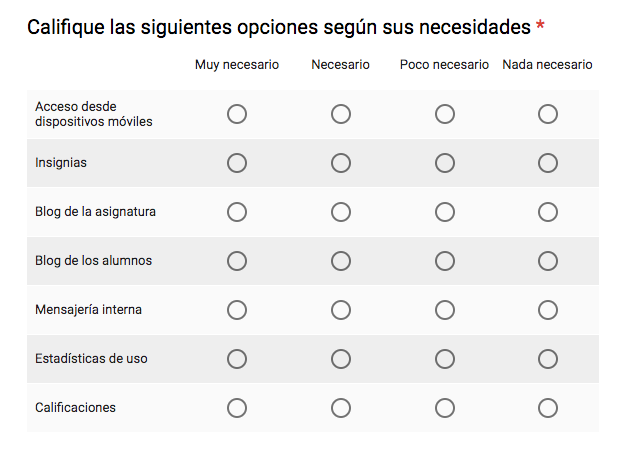
\includegraphics[width=0.9\textwidth]{../screenshots/poll/04}}


  \item \textbf{Actividades y recursos} Presentamos la lista de actividades que puede crear un profesor en una asignatura para ver cuáles son las más utilizadas (las actividades marcadas con * son actividades desarrolladas expresamente para Prado2).


        \begin{itemize}
            \item \textbf{Auto-selección de Grupo *} Esta actividad permite a los alumnos seleccionar su grupo de prácticas al inicio del curso.

            \item \textbf{Base de datos}: Les permite a los participantes crear, mantener y buscar dentro de un banco de entradas de registros.

            \item \textbf{Chat}: Les permite a los participantes tener una discusión sincrónica en tiempo real.

            \item \textbf{Consulta}: Un profesor hace una pregunta y especifica una variedad de respuestas de opción múltiple.

            \item \textbf{Control de Asistencia *}: Esta actividad permite controlar la asistencia a clase.

            \item \textbf{Cuestionario}: Permite al profesor diseñar exámenes, que pueden ser calificados automáticamente.

            \item \textbf{Encuestas predefinidas}: Para recolectar datos de los estudiantes, para ayudar a los profesores a conocer sus alumnos y reflexionar sobre su enseñanza.

            \item \textbf{Foro}: Permite a los participantes tener discusiones asincrónicas.

            \item \textbf{Glosario}: Permite a los participantes crear y mantener una lista de definiciones, a semejanza de un diccionario

            \item \textbf{Herramienta Externa}: Permite a los participantes interactuar con recursos y actividades de enseñanza compatibles con LTI en otros sitios web.

            \item \textbf{Paquete SCORM}: Permite que se incluyan paquetes SCORM como contenido del curso.

            \item \textbf{Lección}: Para proporcionar contenido en formas flexibles.

            \item \textbf{Taller}: Habilita la evaluación por pares.

            \item \textbf{Tarea}: Permite a los profesores calificar y hacer comentarios sobre archivos subidos y tareas creadas en línea y fuera de línea

            \item \textbf{Wiki}: Una colección de páginas web donde cualquiera puede añadir o editar.

            \item \textbf{Archivo}: Son materiales que podemos poner a disposición del alumnado en diferentes formatos: documentos de texto, imágenes, vídeos, audios, archivos comprimidos, etc.

            \item \textbf{Carpeta}: Se utilizan para poner a disposición del alumnado múltiples archivos agrupados en un ítem.

            \item \textbf{Clase grabada (GA3) *}: Esta actividad permite subir una clase grabada con el sistema GA3 para su posterior visualización.

            \item \textbf{Etiqueta}: Se utilizan para insertar pequeñas secciones de texto, imágenes o elementos multimedia entre los distintos bloques de contenido del curso.

            \item \textbf{Libro}: Recursos multi-página con aspecto similar a un libro. Los maestros pueden exportar sus Libros como paquete IMS (el administrador debe permitir que el rol de maestro pueda exportar IMS)

            \item \textbf{Página}: Permiten añadir contenido directamente en Moodle, mediante el editor de texto disponible.

            \item \textbf{Paquete de contenido IMS}: Es un tipo de formato de archivo estándar basado en una serie de especificaciones que facilitan la reutilización de contenidos en distintos sistemas sin necesidad de convertirlos a otro formato.

            \item \textbf{URL}: Permite agregar un enlace a un sitio web.

        \end{itemize}
		\shadowbox{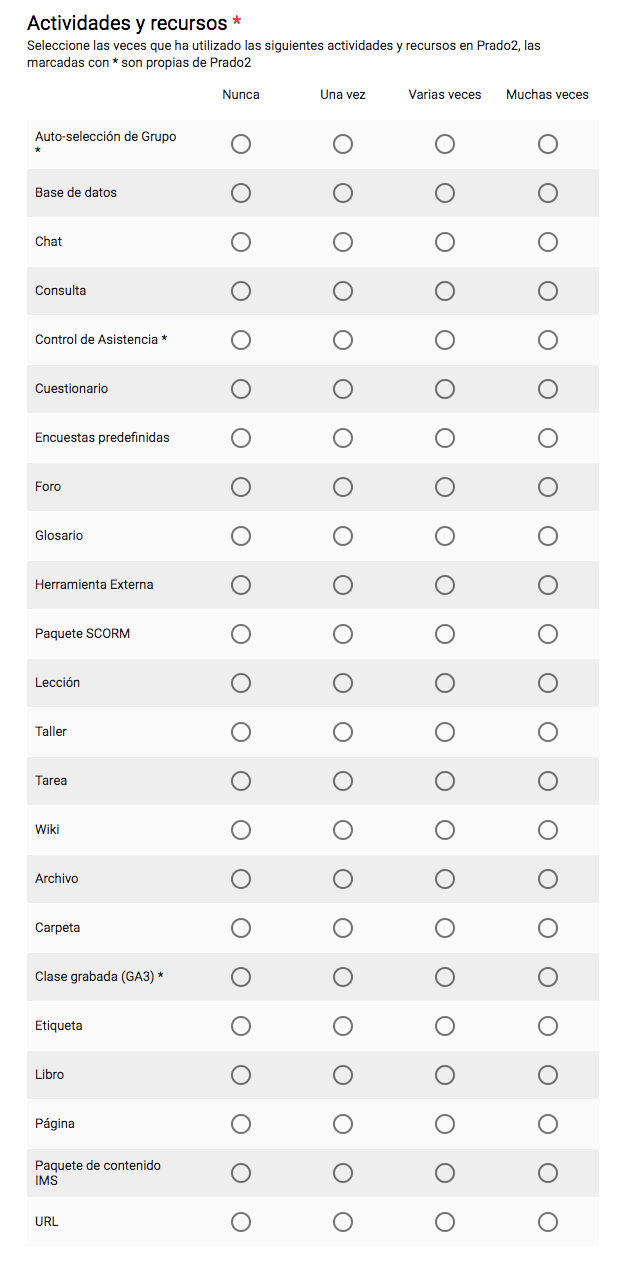
\includegraphics[width=0.9\textwidth]{../screenshots/poll/05}}


  \item \textbf{¿Cómo calificaría Prado2?} Presentamos al usuario los aspectos mas importantes para calificar la plataforma, dichos aspectos son:

  		\begin{itemize}
  			\item \textbf{Usabilidad} Define si un sistema es sencillo de usar, facilita la lectura, presenta funciones y menús sencillos, por lo que es cómodo su uso.
  			\item \textbf{Accesibilidad} Grado en el que todas las personas pueden utilizar el servicio, independientemente de sus capacidades técnicas, cognitivas o físicas.
  			\item \textbf{Seguridad} Define lo robusto que es un sistema frente a ataques informáticos.
  			\item \textbf{Disponibilidad} Disponibilidad: Medida que indica cuanto tiempo está disponible el sistema y lo resistente que es frente a caídas.
  			\item \textbf{Valoracion General} La valoración de la plataforma en su conjunto.

		\end{itemize}

    \shadowbox{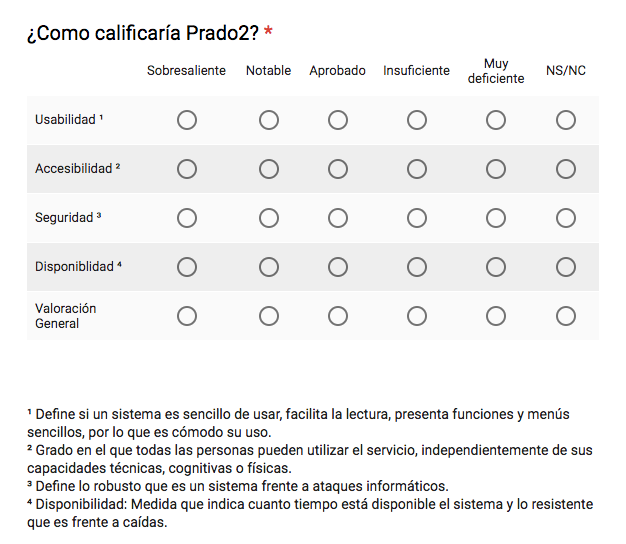
\includegraphics[width=0.9\textwidth]{../screenshots/poll/06}}

  \item \textbf{¿Con cúales de las siguientes plataformas de la UGR ha trabajado?} Presentamos al usuario una lista con las plataformas de docencia más importantes de la UGR:

  		\begin{itemize}
  			\item DECSAI
            \item Tutor
            \item SWAD
            \item Tablón de docencia
            \item Prado 1 - CEVUG (Moodle)
            \item Prado 2 (Moodle)
            \item Otro
		\end{itemize}

  \shadowbox{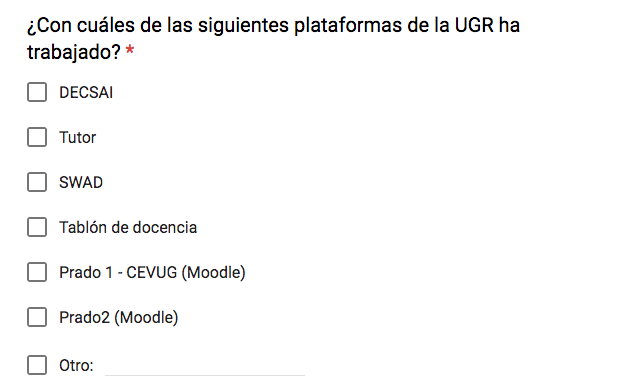
\includegraphics[width=0.9\textwidth]{../screenshots/poll/07}}

  \item \textbf{De las siguientes plataformas de la UGR ¿Cuál prefiere?} Presentamos al usuario una lista con las plataformas de docencia más importantes de la UGR:

  		\begin{itemize}
  			\item DECSAI
            \item Tutor
            \item SWAD
            \item Tablón de docencia
            \item Prado 1 - CEVUG (Moodle)
            \item Prado 2 (Moodle)
            \item Otro
		\end{itemize}

    \shadowbox{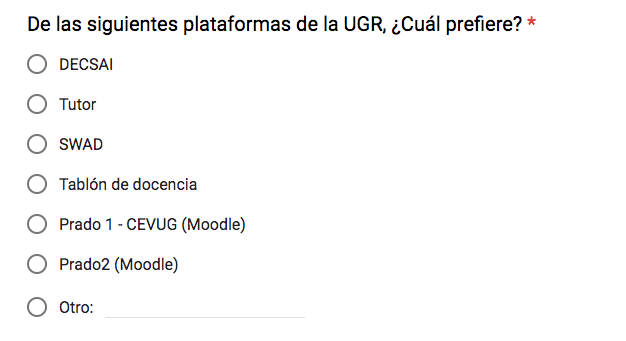
\includegraphics[width=0.9\textwidth]{../screenshots/poll/08}}

  \item \textbf{¿Ha encontrado algún error que debería ser subsanado en Prado2?} Permitimos al usuario expresar su opinión detallada.

  \shadowbox{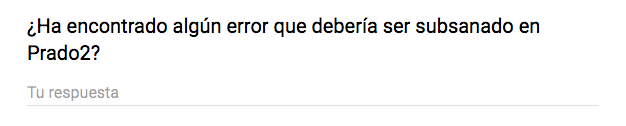
\includegraphics[width=0.9\textwidth]{../screenshots/poll/09}}


  \item \textbf{Indique si hay alguna función adicional que le gustaría ver en Prado2} Permitimos al usuario expresar su opinión detallada.

  \shadowbox{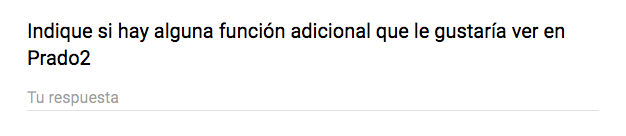
\includegraphics[width=0.9\textwidth]{../screenshots/poll/10}}

  \item \textbf{Indique cuál es la funcionalidad que más le gusta de Prado2} Permitimos al usuario expresar su opinión detallada.

  \shadowbox{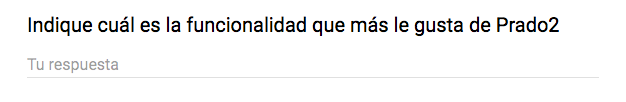
\includegraphics[width=0.9\textwidth]{../screenshots/poll/11}}

  \item \textbf{E-mail} Permitimos al usuario proporcionarnos su dirección de e-mail para futuros contactos.

  \shadowbox{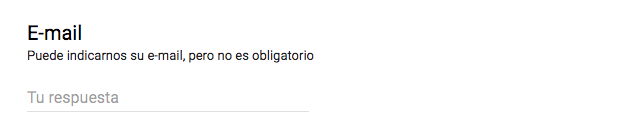
\includegraphics[width=0.9\textwidth]{../screenshots/poll/12}}

  \item \textbf{Comentarios adicionales} Permitimos al usuario expresar su opinión detallada
  
  \shadowbox{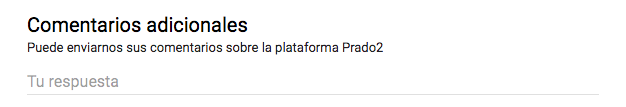
\includegraphics[width=0.9\textwidth]{../screenshots/poll/13}}

\end{enumerate}

\section{Análisis de registros propios de la plataforma}

La plataforma moodle provee de mecanismos para registrar el uso de la misma en diversas tablas de registro, particularmente la versión utilizada usa la tabla \texttt{mdl\_log} (ver figura \ref{logtable}) para almacenar los registros de acceso de los usuarios. Cabe indicar que a partir de la versión 2.7 de moodle la tabla\texttt{mdl\_log}  ya no se utiliza y ha pasado a marcarse como obsoleta\cite{art_09} en favor de la tabla \texttt{mdl\_logstore\_standard\_log}.

Dicha tabla mantiene un registro de todas las interacciones de los usuarios en la página así que podemos extraer información interesante como el tiempo medio de la plataforma por parte de los usuarios o que actividades tienen mas uso. 

Como la tabla contenía información personal como puede ser el identificador del usuario y su dirección ip se optó por diseñar una consulta SQL que retornara los datos usando anonimizando los datos sensibles mediante una función hash.

\begin{figure}\centering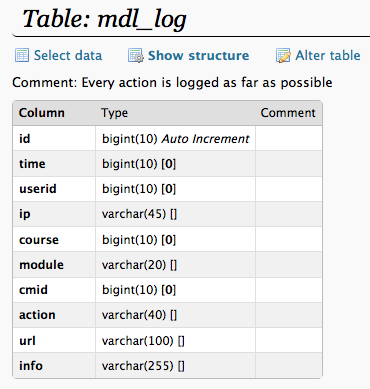
\includegraphics[width=0.8\textwidth]{../images/logtable}\caption{Tabla de log}\label{logtable}\end{figure}

\begin{lstlisting}
SELECT
    id, time, MD5(userid), MD5(ip), MD5(course), module, cmid, action, url, info
FROM
    mdl_log
\end{lstlisting}


Tras una reunión en el CEVUG con los responsables de Prado2 mantenida el 23 de Marzo de 2017 donde nos transmitieron su apoyo y colaboración acordamos realizar una petición formal de datos al CSIRC.

Una vez definida la consulta se realizó al CSIRC una petición formal de datos. Tras varios intentos infructuosos de realizar la petición de forma telemática por parte del tutor se optó por realizarla de forma presencial en papel.

El día 23 de Mayo nos remitieron desde el CEVUG una muestra de los datos de 2014 para ver si los datos eran correctos antes de darnos en fases los datos completos. La primera fase correspondiente a los datos de 2015 los tuvimos disponibles el 1 de Junio en un fichero csv\footnote{Los archivos CSV (del inglés comma-separated values) son un tipo de documento para representar datos en forma de tabla en las que las columnas se separan por comas.} de 500 megabytes conteniendo 3.119.094 registros.


\begin{lstlisting}
SQL> select  /*csv*/ l.id,l.time,rawtohex(sys.DBMS_OBFUSCATION_TOOLKIT.MD5(INPUT_STRING => l.userid)) userid_md5,rawtohex(sys.DBMS_OBFUSCATION_TOOLKIT.MD5(INPUT_STRING => l.ip)) ip_md5 ,l.course, substr(c.idnumber,0,14) course_code,substr(c.idnumber,0,3) tit, substr(c.idnumber,5,2) plan, substr(c.idnumber,8,2) cea, l.module,l.cmid, l.action, l.url, l.info from p_log l, p_course c where (l.course=c.id and l.userid>10 and REGEXP_LIKE(c.idnumber, '^[0-9]') and  l.time>1420070400 and l.time<1451606400);

\end{lstlisting}

Con los datos recogidos y basándonos en el excelente articulo\cite{art_02} de James Ballard que aunque se centra en en el análisis de la nueva tabla de log de las versiones 2.7 y superiores nos sirvió de base con la que crear una serie de consultas en lenguaje R que procesara los datos para sacar conclusiones de los mismo. Dichas consultas se adjuntan en el anexo.

\section{Análisis de usabilidad de la plataforma}

Una vez obtenida la información
Para esta tarea primeramente se tuvieron en cuenta toda la información extraída de las entrevistas personales y se procedió a ver si realmente era usable.

\section{Análisis de accesibilidad de la plataforma}

Se analizó mediante diversas herramientas si la plataforma era accesible, esta tarea la ampliamos para que incluyera tanto la accesibilidad para personas como discapacidad como la accesibilidad desde dispositivos móviles y el uso en otros idiomas.

\section{Análisis de seguridad}

Para analizar la seguridad de la plataforma se realizó una auditoría para ver que información sensible se podía extraer de la misma. Para la misma se analizaron las vulnerabilidades específicas de la versión instalada mirando en distintos repositorios de exploits así como en el propio listado de vulnerabilidades de moodle que se puede encontrar en \url{https://moodle.org/security/}

\bigskip
Asimismo se diseñó un ataque dirigido de secuestro de sesión \textit{(session hijacking)} y se intentaron robar las variables de sesión de moodle del tutor bajo su consentimiento expreso.

\section{Análisis de disponibilidad}

Para el análisis de  disponibilidad de la plataforma se optó por monitorizar la web mediante la herramienta StatusCake \cite{statuscake}.

\bigskip
Dicha herramienta va lanzando continuamente peticiones de conexión a la página desde diferentes centros de datos a lo largo del mundo y va registrando el tiempo que tarda en responder y el tipo de respuesta para saber si la página está operativa o caída.

\bigskip
Una de las cosas interesantes de esta herramienta es que se pueden configurar varios tipos de avisos por lo que si la plataforma sufría una interrupción del servicio nos lo notificaba por e-mail, así como nos notificaba cuando volvía a estar operativo.



\section{Clonado de la plataforma}

Con la información obtenida en en análisis general se planteó la posibilidad de poner un funcionamiento un clon de la plataforma en un servidor propio, en un primer contacto los administradores nos dijeron que lo mismo no sería posible por lo que se optó por realizar una instalación de la misma versión de moodle que hay actualmente en prado así como la plantilla utilizada haciendo las mínimas adaptaciones necesarias para que fuera lo más parecido posible a la instalación actual.

\section{Realización de scripts GreaseMonkey}

Para solventar los problemas de seguridad y accesibilidad se planteó realizar una serie de scripts en formato GreaseMonkey que mediante Javascript pudiera hacer los cambios mínimos para:

  		\begin{enumerate}
  			\item Forzar que la página se sirva mediante el protocolo https.
            \item Realizar simples cambios estéticos para mejorar la usabilidad.
        \end{enumerate}

\section{Herramienta hardware para robo de sesiones}

A modo de ejercicio práctico para ver el alcance de la seguridad de la plataforma se propuso crear un dispositivo hardware para cazar credenciales de usuarios a modo de honeypot utilizando un viejo router instalando el firmware OpenWRT \cite{openwrt} e instalando las herramientas necesarias para obtener los identificadores de sesión de los clientes conectados.



